\subsection{Segmentation}

The main objective of this project was to determine if the physicians/clinicians/technicians are able to obtain more meaningful information when given more depth information.  To give such information structural patterns within the model must be apparent. To achieve this we used a data-set of a human brain containing a tumor. The goal with the depth information inherently found in holography, the location of the tumor will become apparent.  As an intermediate step we need to develop geometry for each of the salient structures of the brain, mainly the white and gray matter, as well as the tumor and other abnormal tissues surrounding the tumor.  This is where segmentation algorithms are needed.\\

There are several different approaches that have been found throughout the literature \cite{pham2000current}.  But they all stem from the same set of core ideas.  Since the brain consists of known tissue types such as white and gray matter, bone and spinal fluid, the intuitive approach would be to classify these based on intensity values of the pixels on the MRI \cite{atkins1998fully}.  The problem arises when there are overlapping tissues and case intensity values of each pixel to be miss classified as one of the known tissue types \cite{undeman2003fully}.  This is why current MRI segmentation is not fully automated and radiologists are needed to help the computer identify which pixels are wrong and correct it. To combat this issue, there are some algorithms such as the one proposed by \cite{lenroot2006brain} whereby they use pre-segmented brain template and perform image registration and automatically identify the troublesome pixels and fix the labels accordingly.\\  

However necessary, the main purpose of this project is not on segmentation rather the depth information of the digital holographic print.  So we will not use complex and accurate segmentation techniques instead we will use the more intuitive approach of pixel classification using multithresholding (MT) techniques \cite{sahoo1988survey} in combination with region growing approaches\cite{adams1994seeded}.\\

The overall goal of MT is to generate masks which partition the image into our desired segmented areas.  To do this a histogram is first to identify the threshold ranges of each tissue type.  The segmentation is achieved by grouping similar pixel intensities together akin to quantizing the images.  But in this case the quantization levels are not constant. This is clearly seen in figure \ref{fig:mriHistogram}.  In the MRI you can see three distinct colours which corresponds to the white and gray matter (WM,GM) and also the cerebral fluid (CSF).  The histogram distributions show 3 distinct peak which corresponds to these tissue types.

\begin{figure}[H]
  \centering
  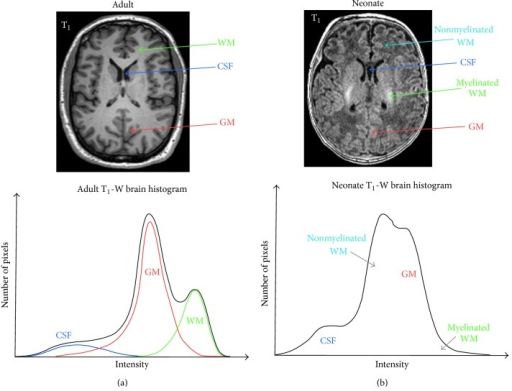
\includegraphics[width=\linewidth]{img/mriHistogram.png}
  \caption{MRI and pixel intensity histogram distribution.}
  \label{fig:mriHistogram}
\end{figure}

Notice the problem described earlier, there are overlapping pixels in the histogram that can be in either of the 3 labeled tissue classes.  We will combat this problem by introducing a region growing approach.\\

Region growing is a simple yet effective technique which samples and extracts a region of the image by connecting similar pixels together. Though very similar to thresholding, this introduces a fuzzy thresholding approach rather than categorical quantization.  The fuzzy approach comes about through the corporation of both the intenisty and edges of the image. The main step is to add a seed point which is manually selected, and from this point connect all the pixels surrounding it together and label that region accordingly.  In the literature this is often done for tumor and lesion segmentation\cite{guliato1998segmentation}. The main disadvantage of this approach is the resultant mask can be very noisy causing the extracted region to have holes and disconnected regions.  To remedy this affect we applied morphological filters\cite{mendiola2007morphological}. 